\documentclass[oneside]{memoir}

\usepackage{lmodern}
\usepackage[T1]{fontenc}
\usepackage[spanish,activeacute]{babel}
\usepackage{mathtools}
\usepackage{graphicx}
\usepackage{titlesec}
\usepackage[document]{ragged2e}
\usepackage{hyperref}
\usepackage{listings}
\usepackage{color}

%Opciones para el formato de los listing
\definecolor{codegreen}{rgb}{0,0.6,0}
\definecolor{codegray}{rgb}{0.5,0.5,0.5}
\definecolor{codepurple}{rgb}{0.58,0,0.82}
\definecolor{backcolour}{rgb}{0.95,0.95,0.92}
 
\lstdefinestyle{mystyle}{
    backgroundcolor=\color{backcolour},   
    commentstyle=\color{codegreen},
    keywordstyle=\color{magenta},
    numberstyle=\tiny\color{codegray},
    stringstyle=\color{codepurple},
    basicstyle=\footnotesize,
    breakatwhitespace=false,         
    breaklines=true,                 
    captionpos=b,                    
    keepspaces=true,                 
    numbers=left,                    
    numbersep=5pt,                  
    showspaces=false,                
    showstringspaces=false,
    showtabs=false,                  
    tabsize=2
}

\lstset{style=mystyle}


\title{YourPlacesBot - A Telegram Bot}
\author{David Quesada L\'opez y Mateo Garc\'ia Fuentes}

\setlength{\parskip}{1em}

\newcommand{\romanpages}{
\pagenumbering{roman}
\thispagestyle{empty}
\beforepartskip
\centering

{\Huge \thetitle}

\theauthor

GRADO EN INGENIER\'IA INFORM\'ATICA 

FACULTAD DE INFORM\'ATICA

UNIVERSIDAD COMPLUTENSE DE MADRID


\includegraphics{logo.jpg}

TRABAJO DE FIN DE GRADO EN INGENIER\'IA INFORM\'ATICA

Director: Carlos Gregorio Rodríguez

\today
\afterpartskip
\newpage

\thispagestyle{empty}
%\beforepartskip
\raggedright

\begin{center}
  \makebox{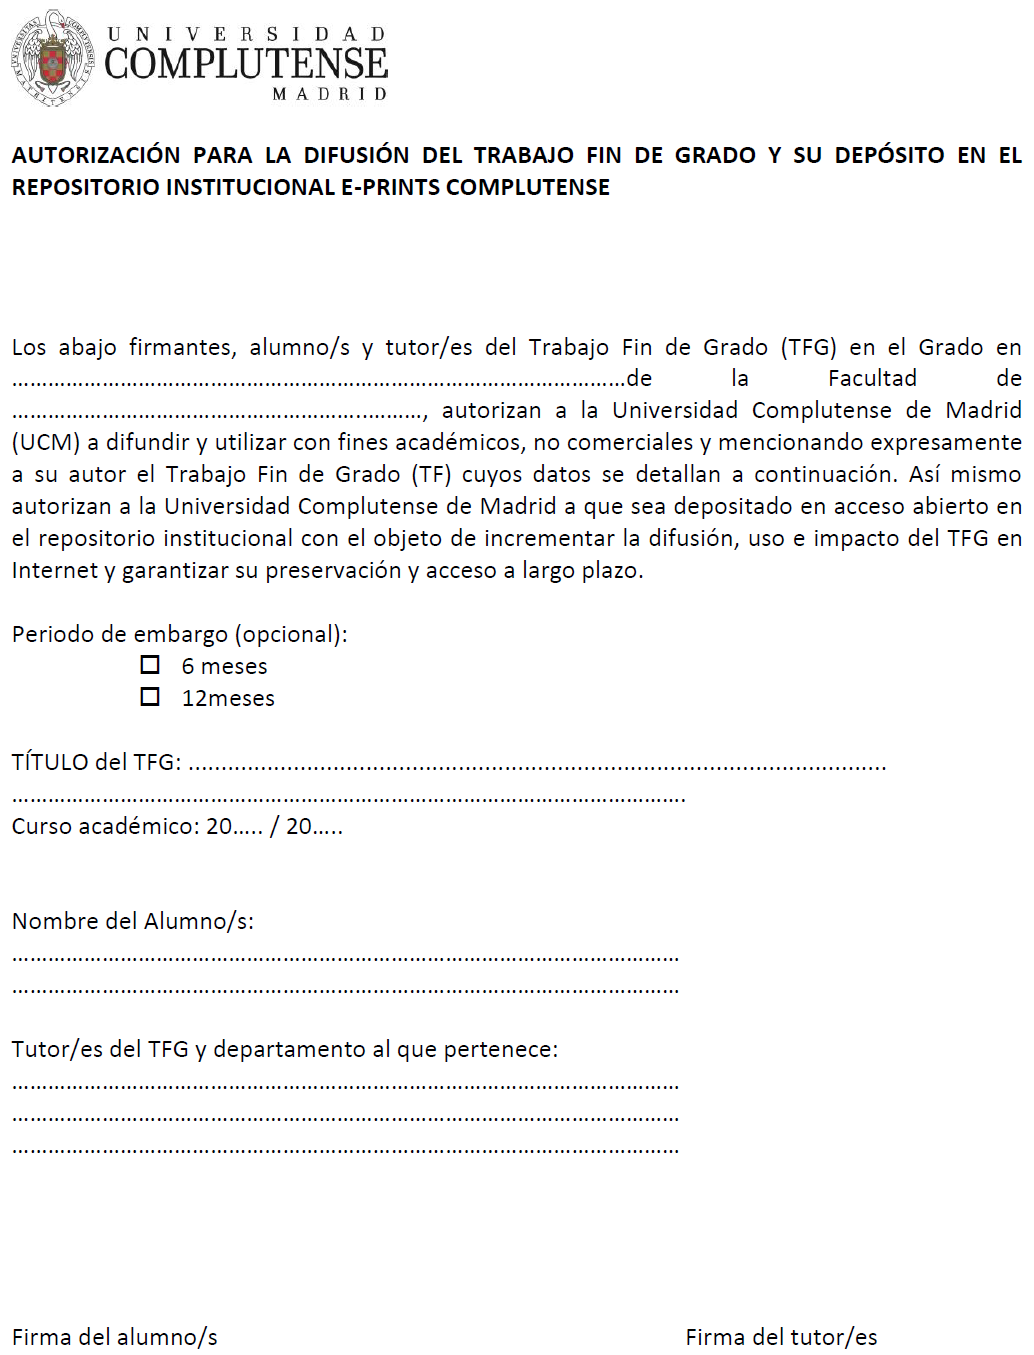
\includegraphics[width=\textwidth]{autoriz.png}}
\end{center}

\afterpartskip
\newpage
\thispagestyle{empty}
\raggedright

\textbf{Agradecimientos}

Gracias a Nick Lee (https://github.com/nickoala) por desarrollar \texttt{Telepot}, un \textit{framework} de \texttt{Python} para la \textit{API} de \texttt{Telegram Bot} y ofrecerlo bajo una licencia \texttt{MIT}.

\afterpartskip
\newpage
}

\newcommand{\indexpage}{
\begin{KeepFromToc}
 \frontmatter
 \setcounter{page}{4}
 \pagestyle{plain}

 \tableofcontents

 \newpage
\end{KeepFromToc}
}

\newcommand{\mychapter}[2]{
    \setcounter{chapter}{#1}
    \setcounter{section}{0}
    \chapter*{#2}
    \addcontentsline{toc}{chapter}{#2}
}


\begin{document}

\romanpages
\indexpage
\mainmatter
\pagenumbering{roman}
\pagestyle{plain}
\justify
\setlength{\parindent}{0pt} %Le he quitado la sangría al documento
\setcounter{page}{5}
\listoffigures
\newpage
\mychapter{0}{\'Indice de abreviaturas}{
\begin{itemize}
\item \textbf{API:} del inglés \textit{Application Programming Interface}, es una interfaz de programación de aplicaciones. Es una definición de los servicios (funciones/funcionalidades) que un determinado módulo \textit{software} provee a otros módulos.
\item \textbf{ESRI:} del inglés \textit{Environmental Systems Research Institute}, es un proveedor de \textit{software} de sistemas de información geográfica (GIS), aplicaciones web de GIS y aplicaciones de gestión de bases de datos geográficas.
\item \textbf{GPL:} del inglés \textit{General Public License}, es una licencia de derechos de autor de \textit{sofware} libre creada por la \textit{Free Software Foundation}.
\item \textbf{GPS:} del inglés \textit{Global Positioning System}, es un sistema de posicionamiento a nivel global que permite determinar la posición de un objeto en nuestro planeta.
\item \textbf{HTTPS:} del inglés \textit{Hypertext Transfer Protocol Secure}, es un protocolo seguro de transferencia de hipertexto. Consiste en la comunicación a través de HTTP (Hypertext Transfer Protocol) dentro de una conexión cifrada que asegura la autenticación del sitio web visitado y la protección de la privacidad e integridad de los datos intercambiados.
\item \textbf{JSON:} del inglés \textit{JavaScript Object Notation}, es un formato de archivo que utiliza texto legible para humanos para transmitir objetos de datos.
\item \textbf{OTAN:} del francés \textit{Organisation du Traité de l'Atlantique Nord}, es una alianza militar entre 28 estados de Europa y Norteamérica.
\item \textbf{QWERTY:} es una distribución de teclado. Su nombre proviene de las primeras seis letras de su fila superior de teclas. Es la distribución más común aunque en algunos países europeos tienen ligeras modificaciones.
\item \textbf{SQL:} del inglés \textit{Structured Query Language}, es un lenguaje de consulta estructurada. Es un lenguaje diseñado para gestionar datos contenidos en un sistema de gestión de bases de datos relacionales.
\item \textbf{PC:} del inglés \textit{personal computer}, son las siglas que denominan un ordenador personal.
\end{itemize}
}

\newpage
\mychapter{0}{Resumen}
\texttt{Telegram} es una aplicación de mensajería instantánea móvil y de escritorio basada en la nube. Esta aplicación, como la mayor parte de las aplicaciones de mensajería instantánea, permite intercambiar mensajes y archivos de todo tipo. En 2016 conseguía llegar a los 100 millones de usuarios y sus servidores procesaban 15 mil millones de mensajes al día \cite{stats}.

Una de los principales atractivos de \texttt{Telegram} es su plataforma para bots. Los usuarios pueden crear sus propios bots y ponerlos en funcionamiento para que sean accesibles a todos los clientes de \texttt{Telegram} sin coste alguno para el desarrollador o para el consumidor. Estos bots proporcionan en su mayoría información, juegos o utilidades dentro de un \textit{chat}, y aumentan en gran medida la funcionalidad de \texttt{Telegram}. 

%Puesto algo sobre asistentes virtuales. No creo que haya que poner mucho más en el resumen, va a pasar de una página si no.
Gracias a esto, hoy en día \texttt{Telegram} no se limita sólo a la mensajería instantánea, sino que también actúa como un asistente personal virtual. Los asistentes virtuales son una característica fundamental en dispositivos móviles, facilitando el día a día de los usuarios y ofreciéndoles información que les es relevante en cualquier momento que lo necesiten. Los bots de \texttt{Telegram} le hacen especialmente potente en este ámbito, ya que continuamente aparecen bots que dotan a \texttt{Telegram} de nuevas capacidades como asistente personal.

A la hora de que un usuario interactúe con un bot, es especialmente interesante que el servicio que se le preste pueda depender de su ubicación geográfica y pueda tener un componente social. Por ello, este proyecto tiene como objetivo informar al usuario sobre qué establecimientos cercanos hay en base a su localización, ofreciendo la posibilidad de encontrarlos fácilmente y de ver datos proporcionados por otros usuarios sobre estos.
\bigbreak
{\Large\textbf{Palabras clave:} bot, Telegram, geolocalización, noSQL, mapas de calor.}

\newpage
\mychapter{0}{Abstract}
\texttt{Telegram} is a cloud-based mobile and desktop instant messaging application. This application, like most instant messaging applications, allows you to exchange messages and files of all kinds. By 2016 it managed to reach 100 million users and their servers processed 15 billion messages a day \cite{stats}. %los billones ingleses no van como los billones españoles, 1 billon inglés = 1000 millones españoles

One of the main features of \texttt{Telegram} is its bot support. Users can create their own bots and launch them to be available for everyone in \texttt{Telegram} without cost for neither the developer nor the client. These bots mainly offer information, games or utilities inside the chat and they increase greatly \texttt{Telegrams} functionality.

This opens the path for \texttt{Telegram} to act not only as an instant messaging application, but also as a virtual personal assistant. Virtual assistants are a vital feature of mobile dispositives, making the user's everyday life easier and offering them relevant information at any time they need it. \texttt{Telegram} bots make it especially powerful in this ambit, given that there are bots constantly being created that offer new personal assistant capabilities.

When an user interacts with a bot, it is of special interest that the response of the bot varies depending on the users location and on a social component. That's why this project aims to inform the user about what near by establishments there are depending on his location, offering the posibility to find them easily and to see information of them given by other users.

\bigbreak
{\Large\textbf{Keywords:} bot, Telegram, geolocation, noSQL, heatmaps.}

\newpage
\pagenumbering{arabic}

\mychapter{1}{Cap\'itulo 1: Introducci\'on}
\section{Motivaci\'on}
Si hacemos un análisis de la sociedad actual es fácil observar que el uso de dispositivos móviles es una constante en el día a día de cada persona. Y que la funcionalidad que ofrecen estos aumenta a una gran velocidad. Estos dispositivos son ya una parte esencial de nuestras vidas, y como consecuencia sus aplicaciones también.

Una de las fortalezas de estos dispositivos es la ayuda que nos ofrecen para procesar toda la información que hay en la red. Las aplicaciones con toda esa información nos ayudan a ampliar nuestra percepción del mundo y a tomar decisiones. Otra de las bazas importantes de las nuevas tecnologías son el carácter social que están adquiriendo, con recomendaciones, fotos, \textit{likes} ... Dentro de estas aplicaciones sociales las de mayor uso son las de mensajería instantánea que nos ponen en contacto con nuestros amigos y conocidos, y nos permiten compartir todo tipo de información.

En algunas de las conversaciones con nuestros amigos había quejas de no disponer de una herramienta sencilla y amigable para encontrar bares, restaurantes y otros tipos de locales de ocio cercanos. En lo primero que piensas para buscar una solución a este problema es en la aplicación de \texttt{Google Maps}. Pero esta aplicación no es cómoda sino está embebida en otra aplicación debido a la enorme cantidad de información que ofrece.

En esta situación, pensamos que un bot de \texttt{Telegram} encajaría bien como solución. Por un lado, \texttt{Telegram} es una aplicación que usamos día a día y un bot resultaría fácil de manejar. Por otro lado, su carácter social nos permite tener un \textit{feedback} con los usuarios que nos permita establecer cuales son las mejores opciones que nos ofrece \texttt{Google Maps}.

\section{Objetivos}
Al empezar este proyecto, la idea principal era crear un bot que funcionase como asistente virtual de los usuarios a la hora de ayudarles a encontrar locales cercanos a ellos. Valiéndonos de la plataforma que nos ofrece \texttt{Telegram}, somos capaces de facilitar el uso de este asistente a millones de usuarios sin tener que preocuparnos de la plataforma en la que lo vayan a usar, ya sean \textit{smartphones}, \textit{tablets} o incluso \textit{pc's}. El bot estará en funcionamiento de manera ininterrumpida y mejorará sus prestaciones en medida del uso que le den otros usuarios, según le vayan aportando nueva información.

De cara a la implementación del bot, este se valdrá de la ubicación que se le envíe para mostrar locales cercanos. Para esto, vamos a establecer una serie de objetivos funcionales que el bot debe cumplir:

\begin{itemize}
  \item Ser capaz de \textbf{recibir una localización} y devolver una serie de locales cercanos a ella. Estos locales deberán estar dentro de un cierto radio de distancia variable y por defecto se buscará que estén abiertos en el instante de la búsqueda.
  \item Cuando se seleccione un establecimiento, \textbf{se devolverá su ubicación} y la información de la que disponga el bot sobre él.
  \item Poderle dar una \textbf{puntuación} a los establecimientos y ser capaz de enviar fotografías al bot.
  \item Poder mostrar un \textbf{mapa de calor} en torno a tu localización reflejando las ubicaciones más concurridas por otros usuarios.
  \item Mostrar \textbf{información} de uso del bot de cara a su posterior desarrollo.
\end{itemize}


\section{Estructura del documento}
Vamos a estructurar este documento conforme al orden en el que fuímos desarrollando el bot. Para cada versión con nuevas funcionalidades, documentaremos qué hemos cambiado, cómo lo hemos hecho y a qué problemas nos hemos enfrentado.

A continuación mostramos sobre qué va a tratar cada capítulo:

\begin{itemize}
  \item \textbf{Capítulo 2: Infraestructura para bots - \texttt{Telepot}}. En este capítulo introduciremos al lector al desarrollo de bots en \texttt{Telegram} contando cómo es la infraestructura que tienen y la \textit{API} que ofrece \texttt{Telegram} a los desarrolladores. También hablaremos de qué es y por qué hemos usado el \textit{framework} de \texttt{Telepot} para nuestro bot en vez de la \textit{API} nativa de \texttt{Telegram}.
	
  \item \textbf{Capítulo 3: Experimentación previa}. Esta parte tratará de nuestro primer acercamiento a la creación de bots. Hablamos de cómo empezamos a usar \texttt{Telepot} para codificar bots simples y lo que aprendimos para usar en un futuro en nuestro bot final.
	
  \item \textbf{Capítulo 4: Primera versión - Establecimientos cercanos}. En este apartado hablamos sobre el desarrollo de la primera versión estable de \textbf{YourPlacesBot}. Esta versión cumple con nuestro primer objetivo que era ofrecer los establecimientos cercanos al usuario. 
  
  \item \textbf{Capítulo 5: Segunda versión - Base de datos e interacción}. Aquí tratamos el desarrollo de la versión que ya era capaz de realizar toda la interacción entre el bot y el usuario. Es la primera versión que pusimos a funcionar de manera continuada en \texttt{Telegram}.
  
  \item \textbf{Capítulo 6: Tercera versión - Opciones y \textit{Heatmaps}}. Este capítulo trata sobre la tercera versión, donde se introducen opciones sobre el funcionamiento del bot que cada usuario puede variar y mapas de calor en base a tu ubicación.
	
  \item \textbf{Capítulo 7: Cuarta versión - Escribir direcciones y estadísticas}. Este apartado trata sobre la última versión del bot, en la cual nuestro objetivo era mejorar y facilitar el uso del bot. Permitiendo al usuario escribir su ciudad, barrio, dirección en vez de tener que mandar la ubicación o comprobar las estadísticas de uso del bot a nivel global.
  
  \item \textbf{Capítulo 8: Conclusiones y trabajo futuro}. En este último capítulo sacamos conclusiones sobre el desarrollo del bot en \texttt{Telegram} y exponemos las mejoras futuras a implementar en el bot.
\end{itemize}

\mychapter{1}{Chapter 1: Introduction}
\section{Motivation}
If we make an analysis of our current society it's easy to observe that the use of mobile devices is a constant in the day to day of each person. And that the functionality they offer increases at a great speed. These devices are already an essential part of our lives, and as consequence their applications too.

One of the strengths of these devices is how they help us processing all the information on the network. Applications with all that information help us broaden our perception of the world and make decisions. Another important asset of the new technologies is the social character that they are acquiring, with recommendations, photos, likes ... Within these social applications the most used are instant messaging that put us in touch with our friends and acquaintances, and allow us to share all kind of information.

In some of the conversations with our friends there were complaints about not having a simple and friendly tool to find bars, restaurants and other types of nearby establishments. The first thing you think to look for a solution to this problem is in the \texttt{Google Maps} application. But this app isn't comfortable unless it's embedded in another applications due to the huge amount of information that it offers.

In this situation, we thought that a \texttt{Telegram} bot would fit well as a solution. On one hand, \texttt{Telegram} is an application that we use every day and a bot would be easy to handle. On the other hand, its social character allows us to have feedback with the users that helps us establish which are the best options that \texttt{Google Maps} offers us.

\section{Objectives}
At the beginning of this project, the main idea was to create a bot that would work as a virtual assistant for users to help them to find places near them. Using the platform offered by \texttt{Telegram}, we are able to facilitate the use of these assistant to millions of users without having to worry about the platform that they'll use, whether they are smartphones, tablets or even pcs. The bot will be in operation in an uninterrupted way and will improve its performance in the measure of the use that other users give it, as they are contributing with new information.

In order to the implement of the bot, this will use the location that it's sent to show nearby establishments. For this, we will establish a series of functional objectives that the bot must comply:

\begin{itemize}
  \item Be able \textbf{to receive a location} and return a series of nearby establishments. This premises must be within a certain radius of variable distance and will be searched by default at the time of the query.
  \item When an establishment is selected , its location and the information that the bot has on it will be returned.
  \item It can give a \textbf{rate} to the establishments and to be able to send photos to the bot.
  \item To be able to show a \textbf{heat map} around your location reflecting the locations most crowded by other users.
  \item To show \textbf{info} of use of the bot for its further development.
\end{itemize}


\section{Structure of the document}
We're going to structure this document according to the order in which we were developing the bot. For each version with new features, we'll document what we have changed, how we have done it and which problems we have faced.

Following is what will treat each chapter:

\begin{itemize}
  \item \textbf{Chapter 2: Infrastructure for bots - \texttt{Telepot}}. In these chapter we'll introduce the reader to the development of bots in \texttt{Telegram} telling how is the infrastructure that they have and the API that \texttt{Telegram} offers to the developers. Also we'll talk what it's and why we have used the \texttt{Telepot} framework for our bot instead of the \texttt{Telegram} native API.
	
  \item \textbf{Chapter 3: Previous experimentation}. This part will deal with our first approach to the creation of bots. We talk about how we start to use \texttt{Telepot} to encode simple bots and what we learned to use in our final bot.
	
  \item \textbf{Chapter 4: First version - Nearby establishments}. In this chapter we talk about the development of the first stable version \textbf{YourPlacesBot}. This version carries out with our first objective that was to offer the the establishments near the user. 
  
  \item \textbf{Chapter 5: Second version - Database and interaction}. Here we treat the development of the version which was already capable of performing all the interaction between the bot and the user. This is the first version that we put to run continuously in \texttt{Telegram}.
  
  \item \textbf{Chapter 6: Third version - Options and Heatmaps}. This chapter deals with our third version, which introduces options about the operation of the bot that each user can change and heat maps based on your location. 
	
  \item \textbf{Chapter 7: Fourth version - Write addresses and statistics}. This chapter is about the latest version of the bot, in which our goal was to improve and facilitate the use of the bot. Allowing the user to type their city, neighborhood, address instead of having to send the location or check the statistics of use of the bot at global level.
  
  \item \textbf{Chapter 8: Conclusions and future work}. In this last chapter we write the conclusions about the development of our \texttt{Telegram} bot and expose the future improvements to be implemented in the bot.
\end{itemize}


\newpage
\mychapter{2}{Cap\'itulo 2: Infraestructura para bots - \texttt{Telepot}}
Para comenzar a desarrollar un bot, hay que familiarizarse con las herramientas que ofrece \texttt{Telegram} para ello. Una vez entendido el funcionamiento de la plataforma de \texttt{Telegram}, de su \textit{API} y de \texttt{Telepot}, estaremos listos para empezar a codificar nuestros bots.
\section{Plataforma de bots de \texttt{Telegram}}
El servicio de mensajería \texttt{Telegram Messenger} ofrece una interfaz de programación para bots, llamada \texttt{Telegram Bot API}. Estos bots son aplicaciones de terceros que se ejecutan en \texttt{Telegram}. La forma de interactuar con estos bots es muy variada: mensajes, comandos, archivos, botones, etc. Las características usuales de estos bots son proporcionar notificaciones y noticias personalizadas, juegos o integración de servicios externos a \texttt{Telegram}.

Los mensajes, comandos y peticiones enviados por los usuarios se envían al \textit{software} que se ejecuta en los servidores. Los servidores de \texttt{Telegram}, que son intermediarios entre nuestro servidor y el usuario, manejan el cifrado y la comunicación. Esta comunicación se realiza a través de una interfaz \texttt{HTTPS} que ofrece una versión simplificada de la \textit{API} de \texttt{Telegram}. 

Los desarrolladores deben crear sus bots a través de \textit{@BotFather}. Este bot es el padre de todos los bots y proporciona \textit{tokens} únicos para cada uno. También es necesario para administrar los bots y gestionar sus configuraciones. Además de esto, el \textit{@BotFather} avisa a los desarrolladores de bots populares (300 solicitudes por minuto o más) si detecta que la tasa de conversión de solicitud/respuesta es muy baja. Está alerta consta de 3 botones de respuesta: Arreglado, Silenciar y Apoyo. Esta última opción abrira un nuevo \textit{chat} con el \texttt{@BotSupport} que ayudará al desarrollador a detectar el problema o averiguar si hay algún problema en los servidores de \texttt{Telegram}.

\begin{figure}[h!]
\centering
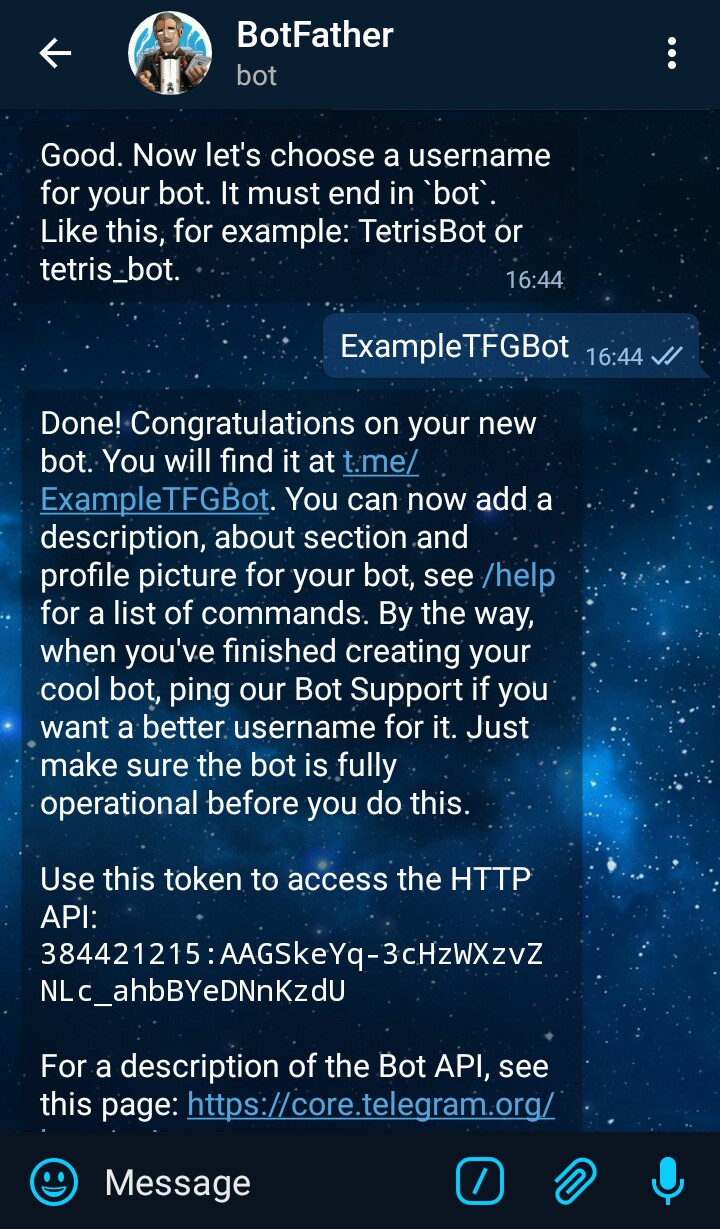
\includegraphics[height=75mm]{tokenBotFather.jpg}
\caption{\textit{@BotFather} provee los \textit{TOKEN}}
\label{fig:tokenBotFather}
\end{figure}

\section{\texttt{Telepot}}
\texttt{Telegram} está desarrollado bajo una licencia GPL \cite{wiki}, es decir, es \textit{software} libre. Por lo que todo el mundo puede ver su código. Esto ha permitido que programadores de todo el mundo hayan creado diversos \textit{frameworks} para la plataforma de bots de \texttt{Telegram} adaptándose a diferentes lenguajes u otras necesidades. 

\texttt{Telepot} es uno de estos \textit{frameworks}, desarrollado por Nick Lee (\url{https://github.com/nickoala/telepot}) te ayuda a desarrollar bots de \texttt{Telegram} usando \texttt{Python}. La funcionalidad básica de \texttt{Telepot} consiste en servir de \textit{wrapper} de todas las funciones de la \textit{API} de \texttt{Telegram} para así poder programar el código de los bots en \texttt{Python}. Como comentábamos en la sección anterior el uso de \texttt{Telegram Bot API} se realiza mediante solicitudes \texttt{HTTPS} a este servicio.

Además de esto, también ofrece funcionalidades para hacer más cómoda la gestión de servidor de tu bot. Cuando creas un bot, tienes que ir pidiendo a los servidores de \texttt{Telegram} \textit{updates} para que te envíen una lista con los mensajes que le han sido enviados. \texttt{Telepot} te proporciona métodos para que no tengas que preocuparte de montar toda una estructura que gestione su recepción. \texttt{Telepot} se encarga de crear hilos de ejecución por cada \textit{chat} nuevo que se abre con el bot y de pararlos cuando estos llevan demasiado tiempo sin realizar ninguna tarea.

Nick Lee ofrece también una guía de referencia de \texttt{Telepot} (\url{http://telepot.readthedocs.io/en/latest/reference.html}) en la que explica en detalle las funciones de las que dispone el \textit{framework}. El uso conjunto del amplio repertorio de ejemplos de código del repositorio de \texttt{GitHub} junto con esta guía de referencia hacen que se agilice bastante el proceso de aprender a codificar bots.

Cabe destacar también que el repositorio está siendo actualizado con frecuencia para adaptarse a las nuevas funcionalidades que va añadiendo \texttt{Telegram}.

\newpage
\mychapter{3}{Cap\'itulo 3: Experimentaci\'on previa}
De cara a afrontar este proyecto, nos encontramos con que debíamos aprender a hacer un bot sin tener conocimientos previos ni de la \textit{API} de \texttt{Telegram} ni de \texttt{Python}. Por tanto, para coger soltura con el lenguaje y con el funcionamiento de los bots dedicamos la primera parte del proyecto a crear bots que realizasen tareas sencillas. Para crear estos bots, fuímos guiándonos del tutorial a base de ejemplos de \texttt{Telepot} (\url{http://telepot.readthedocs.io/en/latest/}).

\section{Creación de los bots}
El primer paso básico para crear un bot es hablar con \textit{@BotFather} para crear tu bot con un nombre y que te envíe el \textit{token} de tu bot. Este \textit{token} es necesario para poder pedirle al servidor de \texttt{Telegram} las \textit{updates} de tu bot. Una vez obtenido el \textit{token}, hay que crear un objeto Bot con el \textit{framework} de \texttt{Telepot} para obtener de manera periódica las \textit{updates} de nuestro bot. Este proceso sería:

\lstinputlisting[language=Python, firstline=58, lastline=61]{Samples/pairingBot.py}

La clase Bot de \texttt{Telepot} es el \textit{wrapper} principal de las funciones en \texttt{HTTPS} de la \textit{API} de \texttt{Telegram} a \texttt{Python}. Llamando al método de \textit{message\_loop} conseguimos que todos los \textit{updates} nuevos los trate la función que le indiquemos por argumento, en este caso \textit{on\_chat\_message(msg)}.

Todos los mensajes que maneja el bot tienen formato \textit{JSON}. Estos mensajes se envían primero a los servidores de \texttt{Telegram}, y son ellos los que se encargan de redirigirlos a su destino. Cuando el bot recibe los mensajes, se puede emplear la función \textit{telepot.glance(msg)} para saber qué contiene (texto, imágenes, audio,...), en qué tipo de \textit{chat} se ha enviado (grupo o privado) y el id de la persona que lo envió. También se puede acceder a esta información accediendo directamente al \textit{JSON} del mensaje.
\lstinputlisting[language=Python, firstline=44, lastline=53, title=Ejemplo de un \textit{on\_chat\_message}]{Samples/pairingBot.py}

\section{Teclados personalizados}
En estos primeros bots también experimentamos con los distintos tipos de teclado que ofrece la \textit{API} de \texttt{Telegram}, los \textit{ReplyKeyboardMarkups} y los \textit{InlineKeyboardMarkups}. La diferencia básica entre estos dos teclados es la posición que ocupan en la pantalla. El primero se sitúa fuera del propio \textit{chat} sitúandose en el lugar que le correpondería al teclado \textit{QWERTY} y el segundo está dentro de la propia conversación obligatoriamente acompañado de un mensaje de texto. Otra diferencia es la manera de procesar las pulsaciones, mientras las pulsaciones a los botones de los \textit{ReplyKeyboardMarkups} se escriben automáticamente en el \textit{chat} como mensaje del usuario, las pulsaciones de los botones de los \textit{InlineKeyboardMarkups} se procesan internamente, cada vez que se pulsa uno de estos botones se crea una clase \textit{ButtonHandler}. Estos botones se procesan como \textit{inline} queries al ser pulsados, de manera que al llegar al bot se diferencian del resto de los mensajes del \textit{chat}.

\begin{figure}[h!]
\centering
\begin{minipage}{6cm}
  \centering
  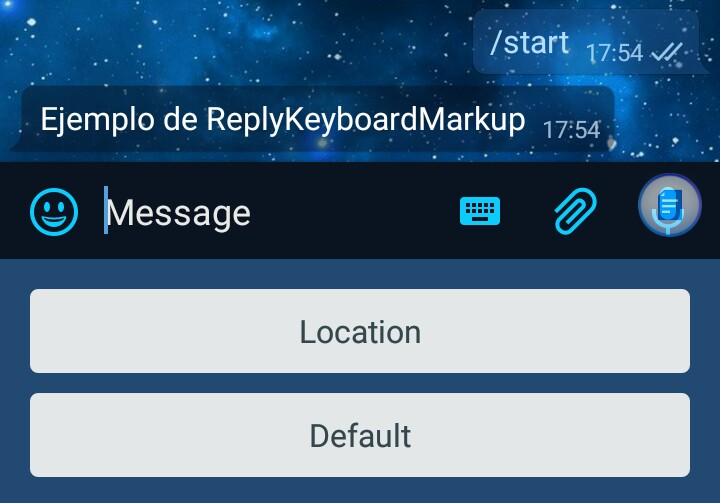
\includegraphics[height=40mm]{replyKB.jpg}
  \caption{ReplyKeyboardMarkup}
  \label{fig:ReplyKeyboardMarkup}
\end{minipage}%
\begin{minipage}{6cm}
  \centering
  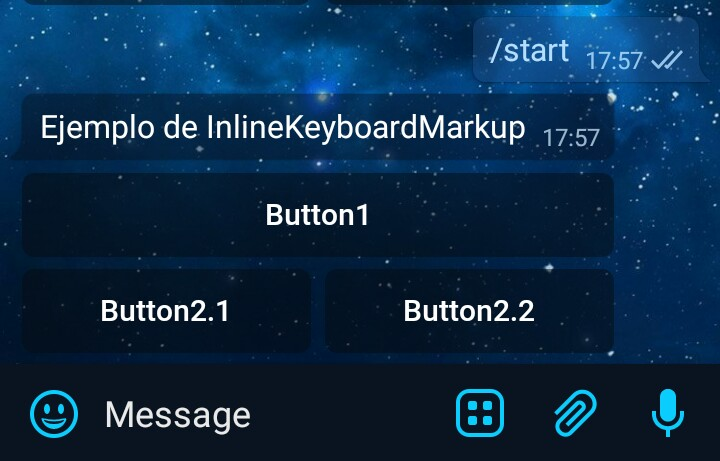
\includegraphics[height=40mm]{inlineKB.jpg}
  \caption{\textit{InlineKeyboardMarkup}}
  \label{fig:InlineKeyboardMarkups}
\end{minipage}
\end{figure}

\section{Gestión de mensajes - \textit{DelegatorBot} y \textit{handlers}}
Lo último con lo que hicimos pruebas en esta primera fase fue con la gestión del servidor. En un principio, nuestros bots procesaban los \textit{updates} que les llegaban de manera secuencial. Cuando ya empezaron a realizar tareas más complejas, tuvimos que crear servidores simples que lanzasen un hilo por cada nuevo \textit{chat\_id} que les llegase en un mensaje. Así, el bot disponía de un diccionario con los \textit{chat\_id} y una cola, para que cada mensaje proveniente de un \textit{chat\_id} ya conocido se encolase para su hilo correspondiente.
\lstinputlisting[language=Python, firstline=82, lastline=87, title=Ejemplo de gestión de mensajes nuevos]{Samples/espiaBot.py}
Tras crear algunos bots que utilizaban este sistema de servidor con hilos por paso de mensajes, nos dimos cuenta de que \texttt{Telepot} proporciona una clase para gestionar todo esto de manera cómoda: la clase \textit{DelegatorBot} y los \textit{handlers}. Esta clase tiene la particularidad de que el objeto bot que creas trata de manera diferente los \textit{updates} que le llegan dependiendo del tipo que sean. Además, este objeto se encarga de lanzar hilos por cada nuevo \textit{chat\_id} que le llega y los tiene todos registrados por debajo en un diccionario, para poder redirigirles los mensajes que les correspondan a cada uno y poder cerrarlos cuando sea necesario.
\lstinputlisting[language=Python, firstline=417, lastline=424, title=Ejemplo de creación de un \textit{DelegatorBot}]{../socialBot.py}
Para gestionar cada mensaje de una forma u otra es necesario definir un \textit{handler} del tipo que corresponda: para gestionar lo relacionado con mensajes en un \textit{chat} se necesita un \textit{ChatHandler} y para tratar las pulsaciones en teclados \textit{inline} se necesita un \textit{CallbackQueryOriginHandler}. Una vez creadas las clases de los \textit{handlers}, debe ponerse un \textit{pave\_event\_space()} por cada tipo de \textit{updates} diferentes que vaya a tratarse. En los argumentos de esta función se especifica qué evento genera un nuevo hilo, en el caso de ejemplo serían \textit{per\_chat\_id()} para el \textit{ChatHandler} y \textit{per\_callback\_query\_origin()} para las pulsaciones en los teclados \textit{inline}. 

El uso del \textit{DelegatorBot} y los \textit{handlers} facilita en gran medida la creación de bots más complejos. Una vez que te acomodas a los diferentes eventos de creación de hilos y de \textit{handlers} que te ofrece \texttt{Telepot}, te ahorra el tener que gestionar tú los hilos y los mensajes, siempre y cuando comprendas bien la gestión interna de estos hilos por parte del \textit{DelegatorBot}.

\section{Repositorio de \texttt{Git} y servidor}
Todos los bots que fuimos desarrollando a lo largo de esta etapa los subíamos a un repositorio privado de \texttt{Git}. Este repositorio era compartido con otros compañeros, que aunque no estaban en nuestro grupo, también desarrollaron un bot de \texttt{Telegram} como Trabajo de Fin de Grado. Para poder tener a los bots funcionando continuamente nuestro director nos proporcionó un servidor, este servidor tiene una clonación (\texttt{git clone}) del repositorio del que estabamos hablando. Por lo tanto sólo no es necesario actualizar la clonación en el servidor una vez que hallamos hecho los cambios en el repositorio, para tener los archivos actualizados.

A parte de este repositorio privado, también creamos un repositorio en GitHub (url{https://github.com/dkesada/SocialBot}) que utilizamos para desarrollar en conjunto nuestro bot. Ahí están recogidos todos los \textit{commits} que hemos ido haciendo así como todo el código del bot bajo una licencia \texttt{MIT}.

\newpage
\mychapter{4}{Cap\'itulo 4: Primera versi\'on - Establecimientos cercanos}
Tras la experimentación previa con \texttt{Telepot} y el desarrollo de varios bots básicos, comenzamos a programar el bot del proyecto. Nuestro principal objetivo en esta primera versión era ofrecer los locales cercanos según la localización que nos ofrecía el usuario.

\section{Funcionalidad básica}
Al iniciar el bot, el usuario recibía un mensaje que rezaba \textit{Share your location!} a la vez que se le ofrecía un \textit{ReplyKeyboardMarkup} con un botón que al pulsarlo compartía la localización del usuario. Después de recibir la localización, el bot continúa preguntando que tipo de establecimiento estaba buscando el usuario, dando varias opciones a través de un teclado \textit{inline}. Cuando el usuario elegía que tipo de local que quería el bot le ofrecía una lista de los establecimientos de ese tipo a un radio de 500 metros. El usuario elegía entre alguno de los locales ofrecidos y el bot le mandaba la localización de este. 

\begin{figure}[h!]
\centering
\begin{minipage}{6cm}
  \centering
  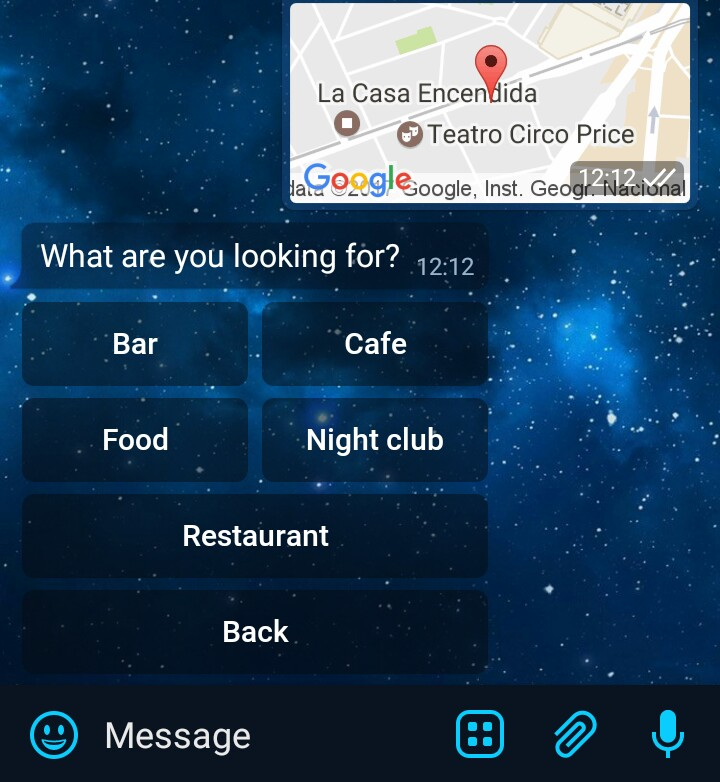
\includegraphics[height=40mm]{paso1v1.jpg}
  \caption{Enviar localización}
  \label{fig:Paso1v1}
\end{minipage}%
\begin{minipage}{6cm}
  \centering
  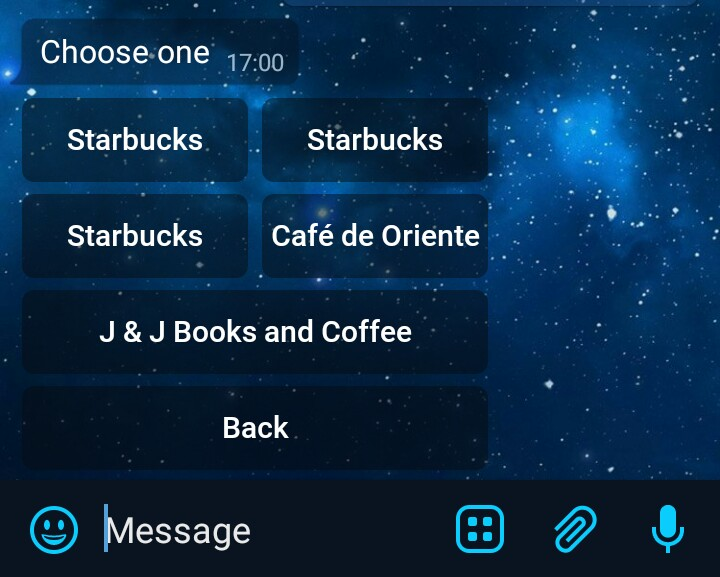
\includegraphics[height=40mm]{paso2v1.jpg}
  \caption{Escoger tipo}
  \label{fig:Paso2v1}
\end{minipage}
\end{figure}

\section{Uso de la \textit{API} de \texttt{Google Maps}}
Para conseguir los establecimientos en un radio de una localización concreta decidimos utilizar el cliente que proporcionan los servicios de \texttt{Google Maps} para \texttt{Python} \cite{Google}. Utilizamos la función \textit{places\_nearby} que al pasarle como parámetros distintos aspectos de la consulta como la localización, el radio, el tipo de local, etc. devolvía una lista en formato \textit{JSON} con todos los establecimientos, y sus datos, que cumplían los parámetros establecidos. Al recibir estos datos nos encargamos de procesarlos para mostrar parte de esta información a los usuarios. 
\lstinputlisting[language=Python, firstline=68, lastline=68, title=Consulta a la \textit{API} de \texttt{Google Maps}]{./Samples/pairingBot.py}%Esta funcion es places no places_nearby
Decidimos usar los servicios prestados por \texttt{Google Maps} por ser la mayor aplicación a nivel mundial que ofrece las geolocalizaciones (entre otros datos) de establecimientos de ocio. Para poder utilizar estos servicios, tuvimos que registrarnos en \texttt{Google Developers} para obtener una clave de la \textit{API} del maps de manera gratuíta con un límite de 1000 consultas diarias.

\begin{figure}[h!]
  \centering
  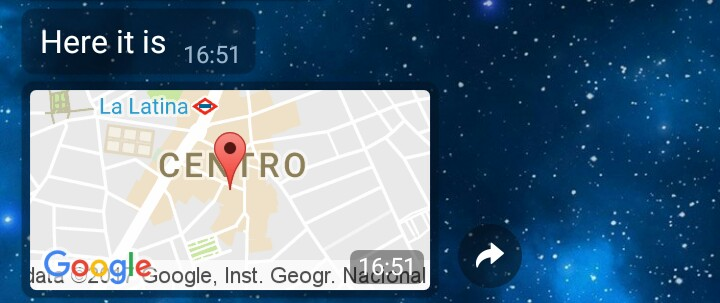
\includegraphics[height=40mm]{paso3v1.jpg}
  \caption{Escoger local}
  \label{fig:Paso3v1}
\end{figure}

\section{Limitaciones de \texttt{Telepot}}
En este punto nos dimos cuenta de una de las limitaciones del los \textit{handlers}. Al definirlos en la llamada a \textit{DelegatorBot}, también hay que poner qué \textit{timeout} tienen. Una vez pasado este tiempo y si el \textit{thread} de un \textit{handler} no ha recibido ningún \textit{update}, el \textit{DelegatorBot} para ese hilo y destruye el objeto \textit{handler} que hubiese. Si después de esto llegase un \textit{update} en el mismo \textit{chat} del hilo que se paró, se crearía un nuevo objeto \textit{handler} y se lanzaría en un nuevo hilo. Esto supone que si se declaró algún atributo privado en el \textit{handler} este se perdió durante el \textit{timeout}, por lo que hay que tenerlo en cuenta y guardar todos los datos relevantes de los \textit{handlers} en la función \textit{on\_time\_out()} definidas dentro de la clase del \textit{handler} correspondiente, que es la que \textit{DelegatorBot} llama antes de hacer el \textit{timeout}.

Otro problema que observamos era que el uso del bot iba llenando el \textit{chat} de mensajes y botones. Pero queríamos conseguir que la interfaz del bot se desarrollase en un solo mensaje y así evitar también que el usuario pueda pulsar botones de manera inesperada. Para mantener el flujo de interacción con el bot por medio de botones \textit{inline} utilizamos continuamente la función \textit{editMessageText} proporcionada por \texttt{Telepot}. Esta función es un \textit{wrapper} de la función de la \textit{API} de \texttt{Telegram} que permite editar un mensaje enviado anteriormente y cambiar su texto y el teclado que proporciona.
\lstinputlisting[language=Python, firstline=96, lastline=96, title=Edición de mensajes previos]{Samples/3rayaBot.py}

%tal vez una imagen de un chat con botones sin eliminar frente a uno con ellos eliminados

\newpage
\mychapter{5}{Cap\'itulo 5: Segunda versi\'on - Base de datos e interacci\'on}
A medida que íbamos desarrollando el bot nos encontrabamos con los primeros problemas, observabamos la necesidad de almacenar los datos y además queríamos mejorar la interacción con el bot para poder establecer un \textit{feedback} con los usuarios.

\section{\texttt{MongoDB}}
Como indicabamos en el capítulo anterior el uso del \textit{DelegatorBot} tenía el inconveniente de perder los atributos privados si no hay actualizaciones en un período determinado. Además queríamos guardar datos como las localizaciones que nos enviaba el usuario para utilizarlos en funcionalidades posteriores. Ante esta coyuntura decidimos crear una base de datos para el bot, algo indispensable en casi cualquier aplicación. La problemática con la que nos encontrábamos era si utilizar una base de datos relacional o no. Nuestra decisión final fue utilizar \texttt{MongoDB}, porque nos ofrecía la capacidad de almacenar nuestros datos que no tenían la misma estructura, pero si parecida, de una manera cómoda. Además nos permitía una futura escalabilidad de esas semi-estructuras que sabíamos que íbamos a necesitar con las futuras funcionalidades del bot. 

Para gestionar la base de datos con el bot implementamos un nuevo módulo utilizando \texttt{Pymongo}, que es una librería de \texttt{Python} que ayuda a gestionar las bases de datos con \texttt{MongoDB}. Dentro de la nueva base de datos establecimos dos colecciones, una de usuarios y otra de establecimientos. Estas dos colecciones no implementan funciones \textit{join}, dado que en \texttt{MongoDB} y en \textit{NoSQL} en general son muy lentas. El bot cuando quiere guardar datos o extraerlos de la base de datos llama a una función específica del nuevo módulo, y este se encargará de conectar con la base de datos para extraer o persistir los datos. Para solucionar el problema del \textit{timeout}, cuando este período de tiempo transcurre invocamos al método \textit{on\_close()} que persiste los atributos que van a expirar en la base de datos.

\section{Interacción con el usuario}
Llegados a este punto, aumentamos la funcionalidad del bot para que una vez que te enviase la localización de algún local también te diese más opciones a realizar con ella. Pusimos la posibilidad de darle una valoración al local que se haya seleccionado, de cero a cinco estrellas, que también se muestra a la hora de enseñarte los locales cercanos a tí. Introducimos también la posibilidad de mandar imágenes de los locales, de forma que si un local tiene imágenes en la base de datos damos la opción de ir viéndolas a través de la interfaz con botones.

\begin{figure}[h!]
  \centering
  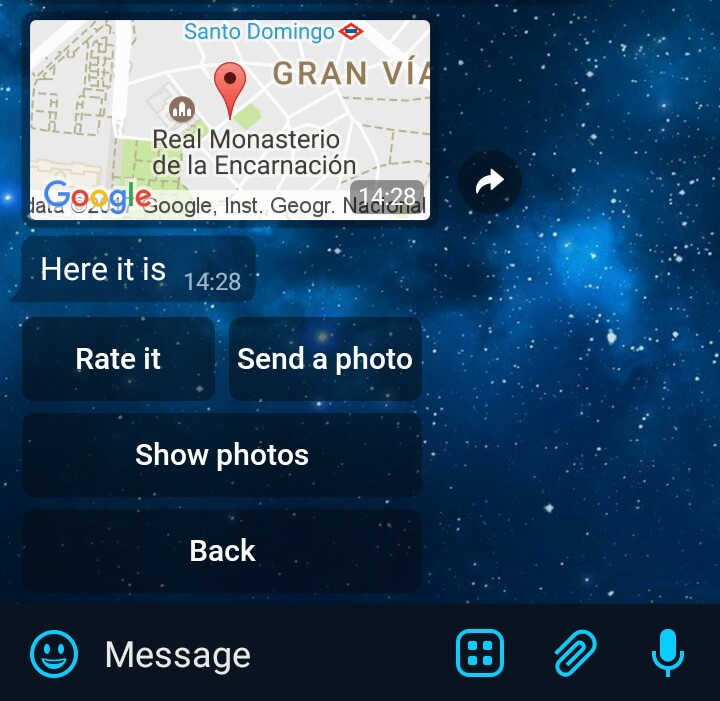
\includegraphics[height=40mm]{interaccionv2.jpg}
  \caption{El usuario puede valorar y ver o envíar fotos}
  \label{fig:interaccionv2}
\end{figure}

Cuando se le envía una imágen al bot, este recibe un \textit{JSON} como si se tratase de un mensaje normal, pero una de las claves contiene el \textit{id} que \texttt{Telegram} le da a la imagen. Es posible descargar el archivo de la imagen si se desea, pero con tener esta clave se puede reenviar y se recibirá como una imagen normal. De este modo, sólo es necesario guardar el \textit{id} de las imágenes que se reciben en el documento de su local correspondiente. Usar \texttt{MongoDB} viene bien es este caso para poder guardar dentro de una misma colección documentos con distintas claves, ya que puede haber locales que no tengan puntuación o imágenes mientras que otros sí.

También para mejorar y dar más información sobre los locales a los usuarios, les proporcionamos la distancia a la que están respecto a su posición actual. Para calcularla utilizamos la fórmula del \textit{haversine} que es una ecuación que calcula la distancia entre dos puntos de un globo sabiendo su longitud y su latitud. Esta función es sólo una aproximación, porque la Tierra no es una esfera perfecta, sino que su radio varía ascendentemente desde los polos hasta el ecuador debido a la forma geoidal del planeta \cite{haversine}. Como radio utilizamos la media geométrica, 6.367,45 kilómetros.

\begin{figure}[h!]
\centering
  \centering
  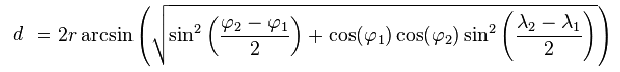
\includegraphics[width=80mm]{hav.png}
  \caption{Fórmula de \textit{haversine} desarrollada para calcular la distancia}
  \label{fig:hav}
\end{figure} 

\section{\textit{Steps}}
Como ahora el bot dispone de más opciones para interactuar con él, también debía disponer de un botón en su interfaz para volver atrás. Como el flujo del bot se desarrolla parecido a una máquina de estados, creamos un módulo \textit{steps} para definir los diferentes estados en los que puede encontrarse el bot, y así saber en cada momento a dónde debe ir en caso de recibir un \textit{update} o de querer volver atrás. Estos estados ayudan también en el caso del \textit{timeout}, ya que en la función \textit{on\_close()} se puede guardar en la base de datos el estado en el que se quedó un usuario, y cuando vuelva pueda continuar usando el bot desde el punto en el que lo dejó. Ahora que disponemos de base de datos, todas las variables locales que utiliza el \textit{handler} también se pueden guardar en caso de \textit{timeout}.

\begin{figure}[h!]
  \centering
  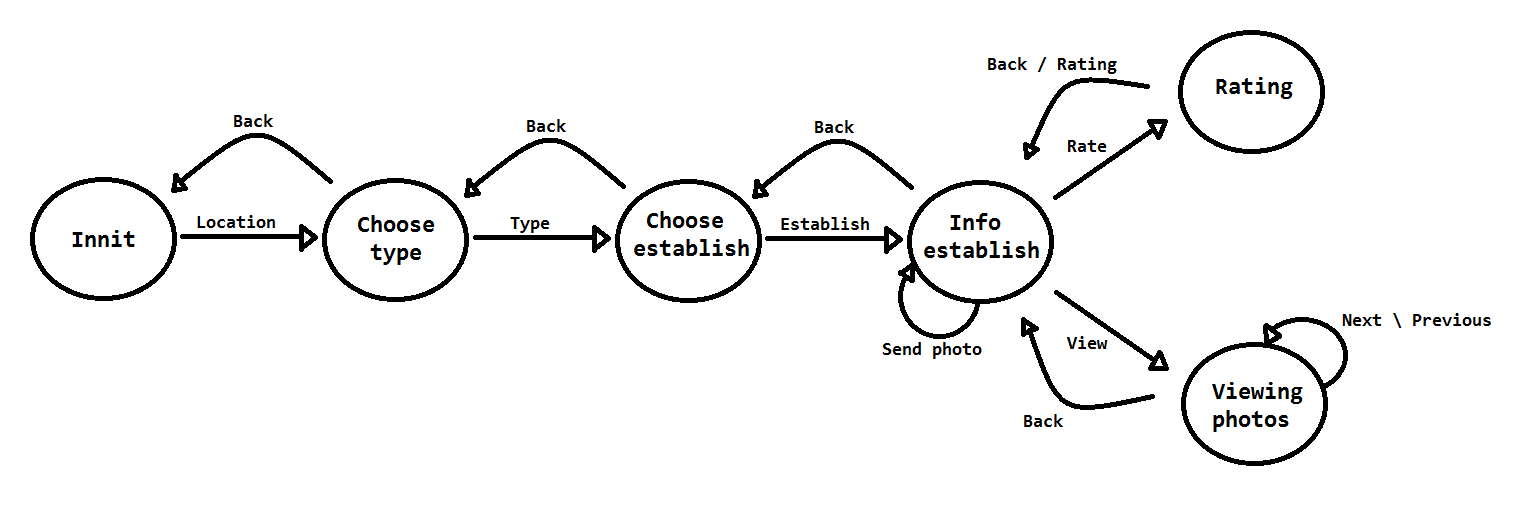
\includegraphics[height=50mm]{steps.png}
  \caption{Estados posibles del bot}
  \label{fig:Estados posibles del bot}
\end{figure}

\section{Otros cambios}
Tras diversas comprobaciones del funcionamiento del bot, observamos que los establecimientos que nos enviaba el método \textit{places\_nearby} no coincidía totalmente con los locales que mostraba \texttt{Google Maps}. Esta consulta no devolvía todos los locales cercanos, sino sólo algunos. Por lo que en su lugar comenzamos a usar el método \textit{places} de la misma \textit{API}, que realiza una búsqueda más exhaustiva. Pasándole por parámetro campos como la localización actual, el radio de la consulta o el tipo de establecimiento que el usuario está buscando. 
\lstinputlisting[language=Python, firstline=181, lastline=181, title=Consulta a la \textit{API} de \texttt{Google Maps}]{../socialBot.py}

% Código de un on_close?
% Mencionar las imagenes en el texto?¿

\newpage
\mychapter{6}{Cap\'itulo 6: Tercera versi\'on - Opciones y \textit{Heatmaps}}
Durante un tiempo estuvimos preparando el bot para que tuviese varios parámetros ajustables en cuanto a su funcionalidad. La \textit{API} de \texttt{Google Maps} permite cambiar opciones de búsqueda como el radio de distancia, buscar sólo establecimientos abiertos o buscar establecimientos dentro de un rango de precios. También podíamos poner el bot tanto en español como en inglés. Juntando todo esto, podíamos crear un nuevo menú el en bot donde cada usuario pudiese cambiar estas opciones si lo desea y después lo persistimos en la base de datos.

\begin{figure}[h!]
  \centering
  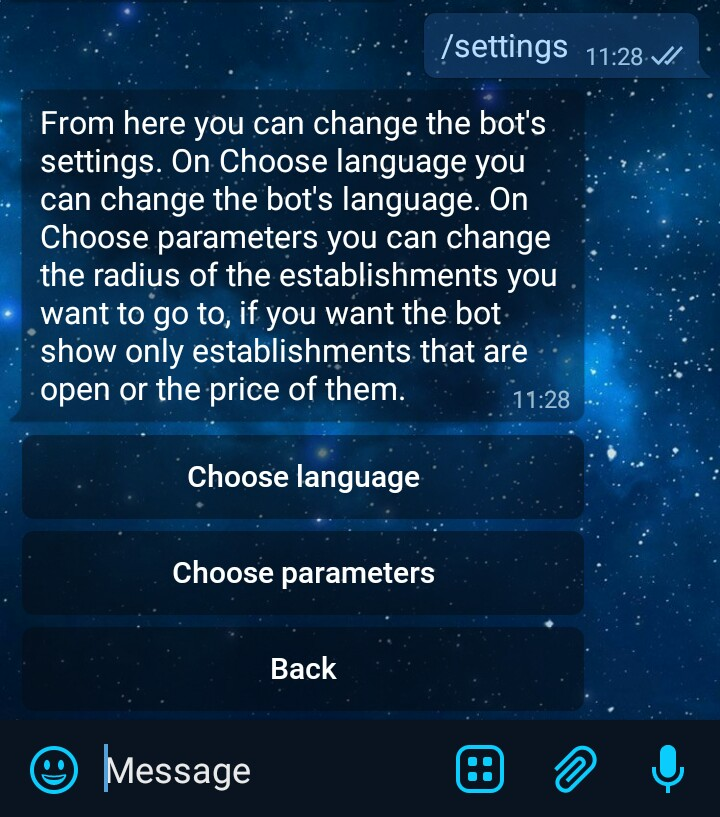
\includegraphics[height=50mm]{settings.jpg}
  \caption{Menú de ajustes}
  \label{fig:settings}
\end{figure}

\section{Idiomas}
Para tener el texto del bot en varios idiomas creamos un nuevo módulo que contiene todos los mensajes de texto y botones que puede enviar el bot. A la hora de enviar un mensaje por el bot, para introducir el texto se hace una llamada a la función correspondiente de este módulo y se le pasa por parámetro una variable que determina si el texto se devolverá en inglés o en español. Por defecto, el bot enviará los mensajes en inglés y podrá cambiarse desde las opciones a español. Para añadir nuevos idiomas al bot, habría que traducir los métodos dentro del módulo \textit{translate.py} y añadir la opción con el nuevo idioma en las opciones del bot. De este modo resulta cómodo poder añadir nuevos idiomas al bot.

\begin{figure}[h!]
\centering
\begin{minipage}{6cm}
  \centering
  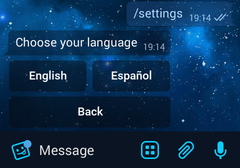
\includegraphics[height=40mm]{elegirIdioma.png}
  \caption{Elegir idioma}
  \label{fig:elegIdiom}
\end{minipage}%
\begin{minipage}{6cm}
  \centering
  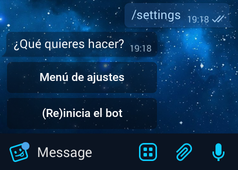
\includegraphics[height=40mm]{esp.png}
  \caption{Tras cambiar a español}
  \label{fig:esi}
\end{minipage}
\end{figure}

\section{Opciones}
De los parámetros variables de la función \textit{places}, al final dejamos el radio de búsqueda, el número de establecimientos que se muestran en una búsqueda y buscar sólo establecimientos abiertos en el momento. 

\begin{figure}[h!]
  \centering
  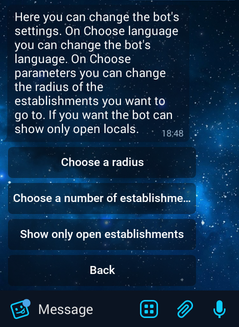
\includegraphics[height=50mm]{parametros.png}
  \caption{Opciones variables del bot}
  \label{fig:parametros}
\end{figure}

La opción de buscar establecimientos según un rango de precios de 0 a 4 daba resultados inesperados cuando la estuvimos probando. Al usar esta opción a veces no mostraba casi ningún establecimiento a pesar de ponerle que buscase en todo el rango, de 0 a 4. Suponemos que esto se debe a que algunos establecimientos no tienen información acerca del rango de precios en el que están, y por tanto no aparecían en búsquedas que usasen ese parámetro. Por tanto, dado que resultó ser menos útil de lo esperado, decidimos no añadir esta opción al bot.


\section{\textit{Heatmaps}}
El cambio más grande de funcionalidad que introdujimos en esta versión fue la capacidad de envíar mapas de calor al usuario. Para recibirlo el usuario debe introducir el comando \textit{/heatmap}, y el bot generará y enviará una imagen con un mapa de calor, cuyo centro es la última localización guardada del usuario que hace la petición. En este mapa de calor se muestran las zonas con más concurrencia cerca del usuario, usando las localizaciones de todos los usuarios.

Para realizar los mapas utilizamos el paquete de \texttt{Python} \texttt{Basemap}, que es una librería para trazar mapas 2D. Permite trazar contornos, imágenes, vectores, líneas o puntos en las coordenadas que se le proporcionen. Para construir el mapa es necesario proporcionarle a la librería los puntos geográficos que corresponden con la esquina inferior izquierda y la esquina superior derecha. Para calcular estos límites, teniendo en cuenta que conocemos el centro de la imagen, utilizamos la fórmula de \textit{haversine} pero a la inversa \cite{inverso}. Si recapítulamos, recordamos que utilizabamos \textit{haversine} para calcular la distancia entre dos puntos en un globo. Nosotros en este caso conocemos uno de los puntos, el ángulo y la distancia, por tanto si despejamos nuestra nueva incógnita tenemos como resultado, lo siguiente:
 
\lstinputlisting[language=Python, firstline=59, lastline=60, title=\textit{Haversine} inverso en \texttt{Python}]{../socialBot.py}

La funcionalidad básica de \texttt{Basemap} sólo ofrece mapas dibujados, lo cúal no nos interesa porque queríamos mayor precisión a nivel ciudad o incluso barrio. Pero sí ofrece la posibilidad de sustituir estos dibujos por otras imagénes. Índicando un código \textit{EPSG}, acrónimo de \textit{European Petroleum Survey Group}, que indican sistemas de referencia de coordenadas. En nuestro caso usamos el código 4326 que indica el sistema \textit{World Geodetic System 1984} en el que está proyectado todo el planeta. Este sistema es usado por los \textit{GPS} y por sistemas militares desarrollados por la \textit{OTAN}. Y para obtener las imágenes vía satélite utilizamos el servicio \texttt{ArcGIS}, de \textit{ESRI}, en concreto el \textit{World Imagery} que tiene 24 niveles de resolución y imágenes en alta definición de casi todo el planeta.

\lstinputlisting[language=Python, firstline=81, lastline=82, title=Consultas a \texttt{Basemap} y a \texttt{ArcGIS}]{../socialBot.py}

%img de heatmap
\newpage
\mychapter{7}{Cap\'itulo 7: Cuarta versión - Escribir direcciones y estadísticas}
Con la tercera versión ya cumplíamos los objetivos que habíamos establecido antes de empezar con el desarrollo del bot. En esta nueva versión nos centramos en hacer más amigable el uso del bot, de manera que el uso sea más rápido y cómodo.

\section{Direcciones}
En anteriores versiones la única forma de que el bot supiera tu localización era compartiéndola o utilizando la que ofrecemos por defecto. En este versión añadimos la posibilidad de escribir la dirección en formato texto, es decir, en el momento en el que el bot te pide la localización el usuario puede escribir la calle, el barrio o la ciudad en la que está. Este texto lo procesamos con la ayuda de otro servicio que ofrece la \textit{API} de \texttt{Google Maps}, \texttt{geocode}, para transformarlo en unas coordenadas geográficas. Mostramos la dirección formateada en la conversación por si hay algún error debido que en distintas ciudades pueden haber calles con el mismo nombre. Y a partir de aquí seguiría el proceso de selección de local de la misma manera que si hubiese compartido la localización.

\begin{figure}[h!]
  \centering
  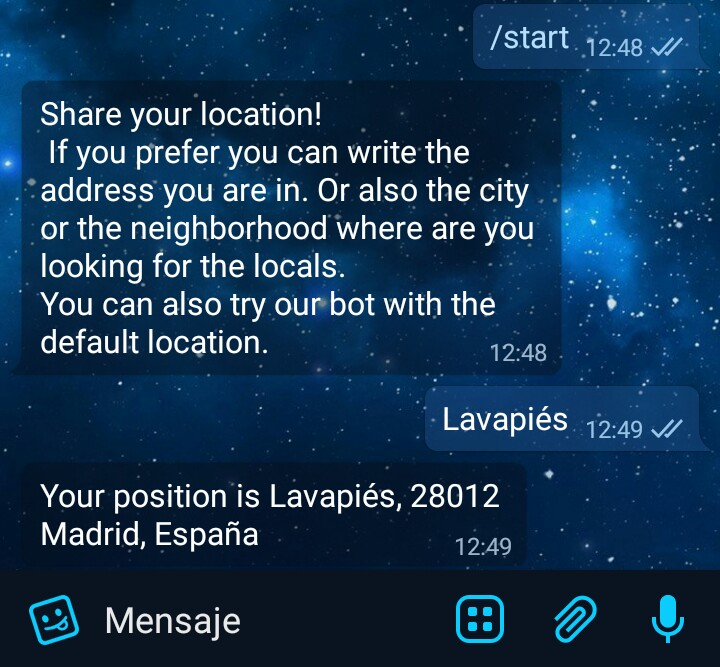
\includegraphics[height=50mm]{direccion.jpg}
  \caption{Envío de dirección escrita}
  \label{fig:direccion}
\end{figure}

\section{Cambios al mostrar los locales}
Anteriormente al mostrar los locales mostrábamos primero en el texto uno por uno todos los establecimientos con la distancia a la que se encontraba el usuario y la puntuación media que tenía y luego una lista de \textit{InlineKeyboardMarkups} de cada uno de los locales. Pero esto en lugares donde hay muchos locales provoca un mensaje muy largo por lo que decidimos cambiarlo. Ya que además como indicabamos en la sección de motivación uno de los problemas que nos encontramos en los servicios para buscar locales de ocio era la gran cantidad de información que nos ofrecían y que éramos incapaces de procesar.

Por ello a partir de esta versión, después de elegir el tipo de establecimiento al que el usuarios quiera ir ofrecemos, por mensaje de texto, los tres locales más cercanos a su posición y los tres mejor valorados por el resto de usuarios en el radio que el cliente tenga establecido. También mostramos la lista  de \textit{InlineKeyboardMarkups} de cada uno de los locales para que el usuario pueda seleccionar el que quiera.

\begin{figure}[h!]
  \centering
  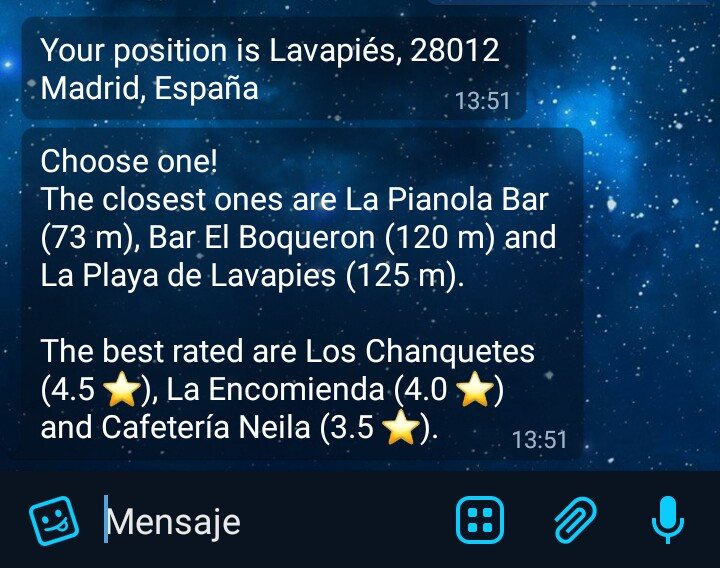
\includegraphics[height=50mm]{muestraLocales.jpg}
  \caption{Cambios al mostrar los locales}
  \label{fig:muestraLocales}
\end{figure}

\section{Estadísticas}
Esta nueva opción solo está disponible para los desarrolladores, se trata de un comando \textit{/stats}, que ofrece las estadísticas de uso del bot. Tras introducir el comando, que no mostramos en la lista de comandos, comprueba si el cliente que introdujo el comando es un superusuario. Los dos únicos superusuarios somos los dos desarrolladores. Si un usuario no autorizado introduce el comando se le enviará un mensaje que le advierte que no tiene permiso para ver ese contenido y se le ofrece la única opción de volver hacia atrás. En el caso de que sí sea un superusuario se muestra el total de usuarios, los usuarios activos durante los últimos siete días, el total de local valorados y los que tienen fotos, también las estadísticas en cuanto al idioma utilizado.

\begin{figure}[h!]
  \centering
  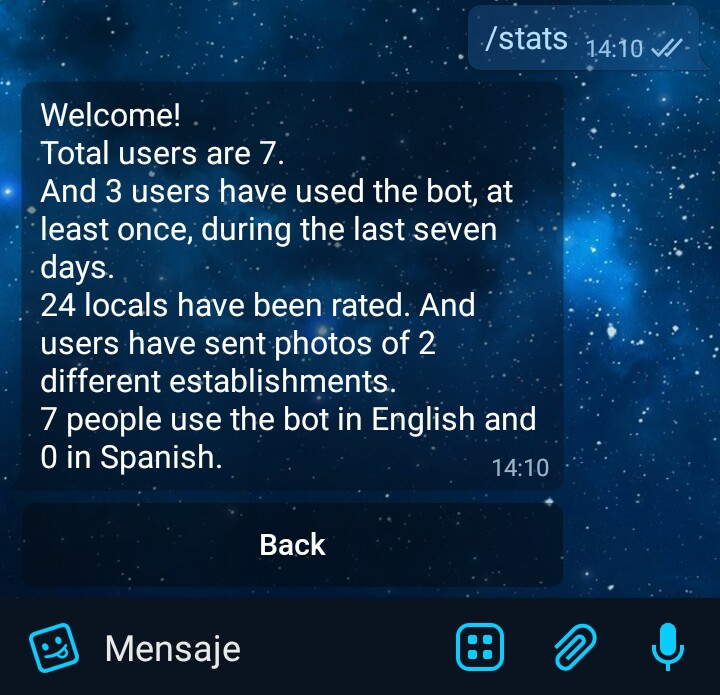
\includegraphics[height=50mm]{stats.jpg}
  \caption{Estadísticas}
  \label{fig:stats}
\end{figure}

\section{Ayuda}
Implementamos un nuevo comando en el bot, \textit{/help}, este comando está presente es casi todos los bots de \texttt{Telegram}. Y su única utilidad es la de resumir como funciona el bot, como utilizarlo y cuales son sus opciones.

\begin{figure}[h!]
  \centering
  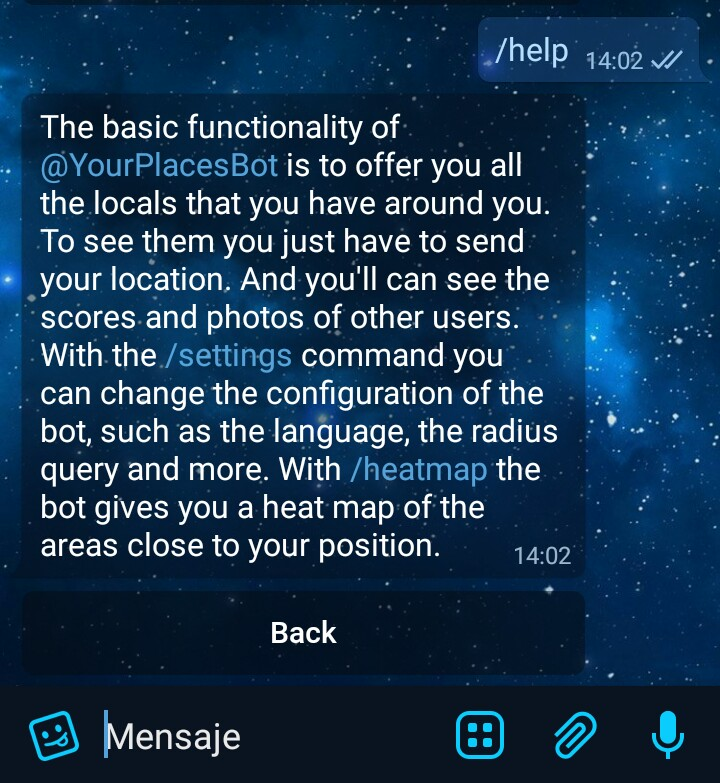
\includegraphics[height=50mm]{ayuda.jpg}
  \caption{Ayuda}
  \label{fig:ayuda}
\end{figure}

\newpage
\mychapter{8}{Cap\'itulo 8: Conclusiones y trabajo futuro}
Finalmente, vamos a recapitular sobre lo que hemos conseguido durante este proyecto de cara a las capacidades adquiridas y a las tecnologías empleadas y sobre el trabajo que queda por realizar en el futuro.

\section{Bots de \texttt{Telegram}}
Al empezar este proyecto, conocíamos los bots de \texttt{Telegram} y habíamos usado alguno antes, pero no sabíamos nada acerca de su creación. De cara a afrontar la codificación del bot, tuvimos que apoyarnos en nuestros conocimientos previos y aprender sobre la marcha las capacidades necesarias. 

Los bots son una herramienta definitivamente potente de \texttt{Telegram}. La capacidad de poder crear herramientas a disposición de millones de potenciales usuarios sin tener que realizar más que unos pocos pasos de creación a través de \textit{@BotFather}, junto con toda la plataforma que te ofrece \texttt{Telegram} ya montada pone a disposición de cualquiera la creación de bots. Esta plataforma ayuda en gran medida a la robustez de los bots, al sólo tener que encargarse de comunicarse con los servidores de \texttt{Telegram} para obtener \textit{updates} y enviar mensajes. 

También es cierto que por ello los bots tienen que adaptarse a la estructura que ofrece \texttt{Telegram}, y hay que ceñirse a las posibilidades de interacción que permite un \textit{chat} de una aplicación de mensajería. A cambio de poder utilizar la interfaz de \texttt{Telegram}, tienes que asumir las limitaciones que presenta. Aún así, compensa adaptarse a su interfaz, ya que ofrece bastantes posibilidades y se van ampliando sus capacidades con bastante frecuencia.

Una vez asumida y comprendida la interfaz, el hecho de estar desarrollando un bot en \texttt{Telegram} se diluye y pasa a ser más un medio que un fin: estás realizando una aplicación que se sirve de la plataforma de \texttt{Telegram} para funcionar, simplemente ciñes la funcionalidad que quieres que tenga tu bot a las posibilidades de interacción que ofrece \texttt{Telegram}, pero por debajo sigue siendo una aplicación que podrías haber adaptado a otro medio distinto.

En definitiva, los bots de \texttt{Telegram} son una muy buena posibilidad a la hora de decidir una plataforma para aplicaciones en dispositivos móviles, dadas las facilidades que ofrecen y la gran visibilidad que puedes llegar a lograr sin coste alguno.

\section{\texttt{Python} y \texttt{Telepot}}
En primer lugar, el lenguaje elegido fue \texttt{Python} para poder aprovechar el uso de \texttt{Telepot}. \texttt{Python} no es un lenguaje ampliamente utilizado durante el grado, por lo que no partimos con conocimientos sobre él. Sin embargo, sí que habíamos usado antes lenguajes orientados a objetos y lenguajes interpretados, por lo que pudimos adaptarnos a él tras el periodo de experimentación previa.

La sencillez al la hora de escribir código en \texttt{Python} hace bastante fácil su aprendizaje y uso, pero su mejor característica es la amplia gama de librerías de las que dispone.

En un principio, el uso de \texttt{Telepot} sólo sirve para codificar los bots en \texttt{Python}, pero una vez comprendido el uso de los \textit{handlers} y de \textit{DelegatorBot}, la carga de trabajo se ve reducida notablemente. 

\section{Base de datos}
Para la base de datos, estamos en un entorno adecuado para \textit{NoSQL}. Dada la diversidad de los datos y el formato \textit{JSON} que utiliza \texttt{Telegram} para hacer llegar los mensajes enviados al bot, resultó una buena opción \texttt{MongoDB}. Esta base de datos orientada a documentos funciona bien fuera del entorno \textit{cluster} al que están dirigidos gran parte de las bases \textit{NoSQL}.

Además, es sencillo integrarlo con \texttt{Python} a través de \texttt{Pymongo}. Como este lenguaje sí lo habíamos practicado antes, pudimos aplicar lo que ya sabíamos de su uso en terminal, dado que el funcionamiento es el mismo que con \texttt{Pymongo}. 

Por ahora no tenemos pensado usar un \textit{cluster} para la base de datos, ya que el tráfico y el tamaño no son suficientes. Aún así, si en un futuro queremos montarlo es posible crear un conjunto de réplica dado que ya partimos de usar \texttt{MongoDB}.

\section{Creación de la memoria}
Durante el grado, nunca nos habíamos enfrentado a la tarea de generar un documento de estas dimensiones y características. Por tanto, de cara a afrontarlo, decidimos emplear \texttt{LaTeX}, un sistema de composición de textos orientado a tareas de este estilo. 

A pesar de que al principio cuesta un poco comprender la sintaxis, después resulta bastante sencillo su uso, dando facilidades a la hora de insertar citas al código y a la hora de estructurar el documento.

\section{Trabajo futuro}
Los objetivos marcados antes del desarrollo del bot los hemos cumplido, pero a medida que se íbamos desarrollando el código nos surgieron nuevas ideas y funcionalidades para añadir al bot, también para mejorar algunas de las partes que del bot.

La idea de añadir reconocimiento de imágenes para que los usuarios nos pudieran enviar fotos de las cartas de comida o bebidas y poder mostrar la información al resto de los usuarios, surgió cuando implementamos la capacidad de poder enviar y ver fotos en el bot. Pero debido a las restricciones temporales tuvimos que decidir si implementar los mapas de calor o el reconocimiento de imágenes, y al final dimos prioridad a los mapas de calor.

Nos gustaría aumentar la funcionalidad de los mapas de calor. Aprovechando el navegador interno de \texttt{Telegram} que permite usar \texttt{HTML5}, poder hacer un navegador sobre un mapa con todos los datos de nuestros usuarios. Es cierto que \texttt{Google Maps} ofrece un servicio parecido en su \textit{API}, pero debido a las restricciones de uso de \texttt{Telegram Bot API} no lo podemos utilizar, ya que no está permitido abrir enlaces externos dentro del navegador. Además nos gustaría ampliar la funcionalidad temporal de los \textit{heatmaps}, es decir, que se pudieran mostrar los mapas de calor según el día elegido o la hora. Para esto también tendríamos que añadir nuevos campos o incluso una nueva colección a nuestra base de datos.

Otra idea que se nos ocurrió pero debido a la falta de tiempo y de datos en nuestra base de datos aún no pudimos implementar eran recomendaciones de locales. Según lo que otros usuarios que hayan valorado con una buena puntuación los mismos establecimientos a los que el usuario también haya dado una buena puntuación, ofrecer otros locales con buenas valoraciones por parte de estos usuarios en los que el usuario aún no haya estado.

Además de esto, como \texttt{Telegram Bot API} es una plataforma que está en continuo crecimiento, con nuevas actualizaciones y nuevas funcionalidades cada cierto tiempo nuestra idea es actualizar el bot a la vez que lo hace la plataforma. E implementaremos nuevas funcionalidades si siguen creciendo las opciones, que sean interesantes para el uso del bot, de la plataforma.

\newpage
\mychapter{8}{Chapter 8: Conclusions and future work}
To conclude, we are going to over what we have acomplished during this project regarding the abilities we acquiered and the technologies we used. We will also talk about the future work that is left to be done.

\section{\texttt{Telegram} bots}
When we began this project, we knew about \texttt{Telegram} bots and we had used some of them before, but we didn't know anything about how they are created. When facing the coding of our bot, we had to rely on our previous knoledge and learn on the fly the necessary skills.

Bots are a definitely powerful tool of \texttt{Telegram}. The ability of being able to create tools that are at the disposition of millions of potencial users by following a few steps through \textit{@BotFather}, along with the platform that \texttt{Telegram} makes it possible for anyone to create a bot. This platform also makes bots more robust, given that you only have to communicate with the \texttt{Telegram} servers to obtain updates and send messages.

However, it's also true that because of this, all the bots have to adapt to the structure offered by \texttt{Telegram}, and you have to stick to the ways of interaction with the user that a \texttt{Telegram} chat offers. In exchange to being able to use the interface of \texttt{Telegram} you have to assume its limitations. Even so, all the posibilities offered by \texttt{Telegram}, which are also being extended with regularity, compensate this.

Once you have comprenhended the interface, you stop thinking about developing a \texttt{Telegram} bot and begin thinking of \texttt{Telegram} as a medium and not as an end. You are developing an application that runs on \texttt{Telegram}'s platform, so you stick the funcionality of your bot to the possibilities of interaction offered by \texttt{Telegram}, but the application you are developing could have been adapted to a different platform.

All in all, \texttt{Telegram} bots are a very good possibility when you think about developing an application for mobile devices, given the advantages they offer and all the visibility that you can achieve without any cost.

\section{\texttt{Python} and \texttt{Telepot}}
When we began this project, we decided to code it in \texttt{Python} in order to be able to benefit ourselves from \texttt{Telepot}. \texttt{Python} is not widely used during the degree, so we had no previous knowledge of it. However, we had used previously object oriented languages and interpreted languages, so we could adapt easily to it after some time.

The easiness of writing code in \texttt{Python} makes learning it very comfortable, but its best characteristic is the wide array of libraries that it has.

At first, using \texttt{Telepot} is only useful to be able to code your bots in \texttt{Python}, but when you comprehend how handlers and the \textit{DelegatorBot} works, it saves you a great amount of work.

\section{Data base}
Regarding the data base, we are in a propper enviroment for \textit{NoSQL}. Given the diversity of the data and the \textit{JSON} format \texttt{Telegram} uses in the bot messages, \texttt{MongoDB} turned out to be a good option. This document oriented data base works well out of the cluster enviroment that most of the \textit{NoSQL} data bases are directed.

In addition, it's easy to integrate it with \texttt{Python} through the \texttt{Pymongo} library. Given that we had already practiced with \texttt{MongoDB} before, we were able to apply what we already knew about its use in terminal with \texttt{Pymongo}.

For now we are not thinking about using a cluster for the data base because its traffic and size are not big enough. Even so, if in the future we want one, it's possible to create a replication set from the data base we already have.

\section{Creation of this report}
During our degree, we never faced the task of writing a document with this length and characteristics. Therefore, in order to tackle it int the best way possible, we decided to use \texttt{LaTeX}, a typesetting system oriented to this kind of tasks.

Even though at fist it takes a while to understand its syntax, after that using it is quite straight forward, making it easy to quote the code and to structure the document.

\section{Future work}
We acomplished the objectives proposed for the bot development, but as we were developing the code we thought of new ideas and functionalities that we could add to the bot and that we could use to improve it.

We thought about adding image recognition so that users could send photos of restaurants menus and then show it to the rest of users. We thought about this when we implemented the image sending and recieving of the bot. But due to time restrictions, we had to decide whether we implemented the heatmaps or the image recognition, and eventually we decided on the heatmaps.

We would like to improve the functionality of the heatmaps. We could use \texttt{Telegram} internal web browser that allows us to use \texttt{HTML5}, and then we could make the heatmap inside that browser. \texttt{Google Maps} offers a similar service in its \textit{API}, but due to the restrictions of using the \texttt{Telegram Bot API} we couldn't use it, because you can't open external links inside the browser. We would also like to make heatmaps depending on the day or the time you want them. To make this possible we would also have to add new information in the data base.

Another idea we had but that we didn't have enough time and user data to implement was stablishments recomendations to users. Comparing what other users have rated positively with what you have, offer stablishments these users have rated and that you havent visited.

On top of this all, given that \texttt{Telegram Bot API} is in continuous development with new updates and new functionalities, our idea was to improve our bot when \texttt{Telegram} offers new interesting ways of interaction.

\setcounter{secnumdepth}{0}% Desabilita la numeración de las secciones
\newpage
\mychapter{9}{Aportaciones individuales}
En general ambos autores hemos participado en todos los aspectos del proyecto. La parte de la experimentación previa la realizamos de forma individual, aunque trabajando aspectos muy parecidos y utilizando \texttt{Telepot}.

\section{David Quesada L\'opez}
Cuando comenzó el proyecto conjunto, monté el repositorio de git que hemos utilizado durante todo el proyecto. Decidí ponerle una licencia \texttt{MIT} como la usada por \texttt{Telepot}, para que si alguien se encuentra con el proyecto y le puede ser de utilidad pueda valerse de él libremente mencionándonos.

Al comenzar a codificar el bot, creé la estructura base del bot a partir de los bots que había desarrollado en la fase de experimentación. Durante esta fase, me había centrado especialmente en el uso de los \textit{handlers}, los \textit{delegator} y los teclados \textit{inline}, por lo que la estructura inicial fue lo bastante robusta como para soportar el resto de la codificación del bot.

Me encargué también de preparar la \textit{API} de \texttt{Google Maps} para poder usarla, registrándose y obteniendo la clave. Hice las primeras pruebas del método \textit{places\_nearby}, aunque en este momento del desarrollo aún no nos dimos cuenta de que este método no funcionaba correctamente. 

Implementé la base de datos en \texttt{MongoDB} con \texttt{Pymongo} en un nuevo módulo. Este nuevo módulo contendría todas las funciones relativas a la interacción con la base de datos. Monté la estructura de lo que empezaríamos guardando en la colección \textit{usuarios}, y dado que usamos \texttt{MongoDB} es fácil cambiarlo en un futuro para guardar nuevos datos o añadir colecciones. Monté también el \textit{script} para lanzar la base de datos en el servidor. 

Junté en otro módulo todos los teclados que utilizamos en el bot, para que fuese más sencillo encontrarlos y realizar cambios en ellos. De esta forma para introducir un teclado a un mensaje lo llamamos como a una función. De cara a la funcionalidad del bot, me encargué de hacer la parte de recibir fotos de cada local y guardarlas en la base de datos. Finalmente, cambié la forma de guardar localizaciones de establecimientos en la base de datos de cara a crear un índice geoespacial en un futuro.

En cuanto a la memoria, comencé escribiendo el resumen y el capítulo 1, montando la estructura que seguiríamos luego. Escribí el capítulo 2 y el capítulo 3, sobre los pasos previos a la creación de nuestro bot. El capítulo de la segunda versión lo escribimos a medias, encargándome yo de las secciones de \texttt{MongoDB} y de los \textit{steps}. En la tercera versión hice las dos primeras secciones. Finalmente, escribí el último capítulo excepto el trabajo futuro. 

\section{Mateo Garc\'ia Fuentes}
En la primera versión, me encargué de procesar los datos que devolvía el método \textit{places\_nearby} de manera que guardaba el nombre y las coordenadas de los locales para así mostrar los restaurantes en botones y al pulsar estos mandar la localización del establecimiento pulsado. Después también me encargué de filtrar los establecimientos por tipo, es decir, el método \textit{places\_nearby} acepta como parámetro unos determinados tipos de locales de los cuales mostramos cinco al usuario y una vez pulsado se le muestran al usuario los establecimientos de ese tipo. 

En la segunda versión, me encargué de iniciar el primer esqueleto de \textit{steps}, aún en el archivo principal, que pasaría a ser un módulo que controla los pasos de cada usuario en el bot. También me encargue de implementar la opción que permite ir hacia atrás a los usuarios, en el módulo \textit{steps} ya separado que se invoca desde un \textit{InlineKeyboardMarkup}. Después de que observamos que el  método \textit{places\_nearby} no ofrecía todos los establecimientos posibles me encargué de cambiar este método por el nuevo \textit{places} que ofrece el mismo servicio de \texttt{Google Maps}. De la nueva parte de la interacción con el usuario me encargué de implementar que el usuario pudiera realizar las puntuaciones del local que haya elegido y que mostrase la puntuación de todos los establecimientos en el paso de elegir local. También me encargué de investigar e implementar la fórmula de \textit{haversine} para calcular la distancia entre la ubicación del usuario y el establecimiento. También implementé  la funcionalidad de mostrar las fotos de los locales que las tuvieran.

En la tercera versión, implementé la funcionalidad de \textit{settings} que son los ajustes que el usuario puede cambiar como el idioma, el radio de las consultas o si solo quiere ver los establecimientos abiertos. También me encargué de que estos ajustes se tuvieran en cuenta en la consulta que hacemos a la \textit{API} de \texttt{Google Maps} donde le introducimo por parámetro los ajuste que tenga seleccionados el cliente. Programé el nuevo módulo de esta versión que era el encargado de traducir el bot, como explicamos anteriormente el bot recibe el idioma del usuario y devuelve la frase correspondiente en el idioma indicado. La mayor parte de la implementación de los \textit{heatmaps} lo hicimos en conjunto, excepto la función \textit{calculateBounds} que se encarga de calcular la esquina inferior izquierda y la superior derecha de la imagen del mapa de calor utilizando la fórmula del \textit{haversine}, como explicamos en un capítulo anterior.

En la cuarta versión, implementé la funcionalidad de ayuda, también añadí la nueva funcionalidad de escribir la dirección por texto con el nuevo método de \textit{geocode}. Además me encargué de mejorar la manera de mostrarle la información de los establecimientos a los usuarios de forma que fuera más amigable para este.

En la memoria, me encargué de explicar los tipos de teclados que ofrece \texttt{Telegram Bot API} y escribí el capítulo de la primera version. De la segunda version expliqué las secciones de interacción con el usuario (valoraciones, \textit{haversine}, ...) y de otros cambios (el cambio al método \textit{places}). En el capítulo de la tercera versión me encargué de explicar como implementamos los mapas de calor. Además también escribí el capítulo de la cuarta versión y el índice de abreviaturas. Tras enviar el primer borrador me encargué de corregir el resumen y la introducion además de los capítulos 2 y 4.

\newpage
\begin{thebibliography}{14}
\bibitem{LaTex}
LaTex -> \url{https://www.latex-project.org/}
\bibitem{Memoir}
The memoir class - User guide -> \url{http://texdoc.net/texmf-dist/doc/latex/memoir/memman.pdf} 
\bibitem{Python}
Python -> \url{https://docs.python.org/2.7/}
\bibitem{Google}
API Google Maps Docs -> \url{http://googlemaps.github.io/google-maps-services-python/docs/2.4.5/}
\bibitem{Telegram Bots}
Telegram Bots -> \url{https://core.telegram.org/bots/api}
\bibitem{Telepot}
API Telepot -> \url{http://telepot.readthedocs.io/en/latest/}
\bibitem{MongoDB}
MongoDB -> \url{https://docs.mongodb.com/manual/}
\bibitem{Pymongo}
Pymongo -> \url{https://api.mongodb.com/python/current/}
\bibitem{Basemap}
Basemap -> \url{https://matplotlib.org/basemap/}
\bibitem{ArcGis}
ArcGis de ESRI -> \url{http://www.esri.com/arcgis/about-arcgis}
\bibitem{stats}
Estadísticas de uso de Telegram -> \url{http://expandedramblings.com/index.php/telegram-stats/}
\bibitem{wiki}
Artículo de Wikipedia de Telegram -> \url{https://es.wikipedia.org/wiki/Telegram_Messenger}
\bibitem{haversine}
Fórmula del haversine -> \url{https://en.wikipedia.org/wiki/Haversine_formula}
\bibitem{inverso}
Haversine inverso desarrollado en Clojure-> \url{https://gist.github.com/shayanjm/451a3242685225aa934b}

\end{thebibliography}


\end{document}
